\subsection{Structures}

\subsection{Unit Construction Structures}


Figure~\ref{fig:struct_units} shows the Markov Chain which dictates the behaviour of unit constructing structures. The unlabelled actions represent the change state change from building a unit to being idle which the player has no control over. The probabilities \(P_{I}\) and \(P_{B}\) refer to the probability that an idle structure remains idle or builds a unit. \(P_{UX}\) refers to the probability of the structure building unit \(X\).

\begin{figure}
\centering
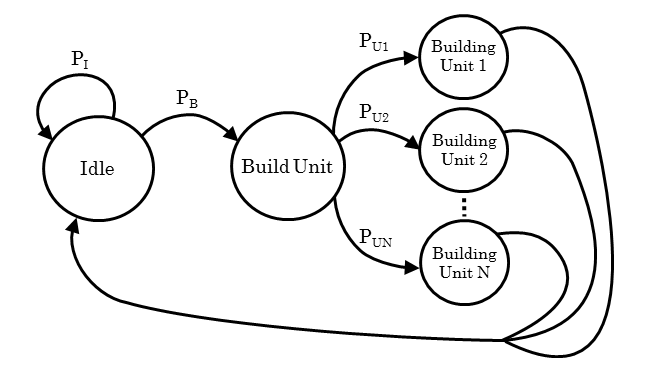
\includegraphics[scale=0.8, trim = 0cm 0cm 0cm 0cm]{diagrams/building_units}
\label{fig:struct_units}
\caption{A generalised Markov chain for unit building structures.}
\end{figure}

\subsection{Research Orientated Structures}

-create a similar generic diagram for research structures

-indicate using states how certain options are cut off

-maybe change the diagram

\begin{figure}
\centering
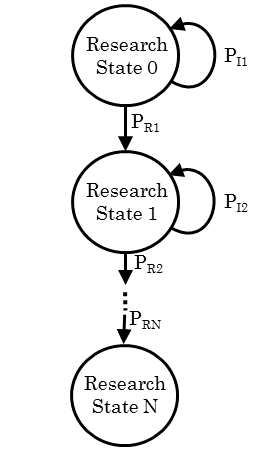
\includegraphics[scale=0.8, trim = 0cm 0cm 0cm 0cm]{diagrams/building_research}
\label{fig:struct_research}
\caption{A generalised Markov chain for unit building structures.}
\end{figure}